\documentclass[conference]{IEEEtran}
\usepackage{graphicx}

% turn off hypenation
\tolerance=1
\emergencystretch=\maxdimen
\hyphenpenalty=10000
\hbadness=10000

\begin{document}

\title{Project Final Report:\\Matrix Profile MPI Implementation}

\author{\IEEEauthorblockN{Brody Larsen\IEEEauthorrefmark{1} and Richard McNew\IEEEauthorrefmark{2}}
\IEEEauthorblockA{Department of Computer Science, Utah State University\\ Logan, Utah, USA\\
\IEEEauthorrefmark{1}a01977457@usu.edu, \IEEEauthorrefmark{2}a02077329@usu.edu}
}


\maketitle
\begin{abstract}
The Matrix Profile is an amazing data structure and set of accompanying algorithms that have revolutionized time series data mining tasks over the past five years.  Most data science work is done in Python.  As a result, most Matrix Profile implementations in use today are written in Python and rely on the NumPy, SciPy, and Numba Python libraries for vector and matrix data types, numerical and scientific algorithms, and fast just-in-time optimizations.  In this project we created an MPI implementation of the Matrix Profile in C++.
\end{abstract}

\begin{IEEEkeywords}
parallel computation, MPI, data science, Matrix Profile, C++
\end{IEEEkeywords}


\section{Introduction}
Time series data is a collection of observations made sequentially in time.  Time series data is ubiquitous in our modern world and takes the form of sensor data, stock market data, network metrics, application logs, and many other forms.  Analyzing time series data is essential to understanding what is happening and enables informed decision-making and strategic planning.  One recent advancement in time series data analysis is the Matrix Profile\cite{MatrixProfile1}. 

The Matrix Profile is an amazing data structure and set of accompanying algorithms that annotate a time series and make most time series data mining problems easy to solve\cite{MatrixProfile2}. The Matrix Profile is:  1) exact - it allows for time series analysis without false positives or false negatives, 2) parameter-free - unlike many time series data analysis tools, no hyperparameter tuning is needed, 3) space efficient - a matrix profile data structure does not require much space, enabling large datasets to be processed in memory, 4) parallelizable - it is fast to compute on modern hardware, and 5) simple - it is easy to use and fairly easy to understand\cite{Keogh}.   

Most data science work is done in Python.  As a result, most Matrix Profile implementations in use today are written in Python\cite{Stumpy} and rely on the NumPy, SciPy, and Numba Python libraries for vector and matrix data types, numerical and scientific algorithms, and fast just-in-time optimizations.  Creating a Matrix Profile implementation using MPI in C++ will offer organizations that use MPI a way to use the Matrix Profile. 

\section{Project Thesis}
In this project we created a minimal MPI-based implementation of the Matrix Profile in C++.

\section{Background}
\subsection{Definitions and Notation}

We must first formally define a \emph{time series}:

\textbf{Definition 1:} A \emph{time series} $T$ is a sequence of real-valued numbers $t_i$: $T = t_1, t_2, \ldots{}, t_n$ where $n$ is the length of $T$.

In most cases, only some parts of the time series are interesting rather than the entire time series.  These \emph{subsequences} are what we want to find and study.

\textbf{Definition 2:} A \emph{subsequence} $T_{i,m}$ of a \emph{time series} $T$ is a continuous subset of the values of $T$ of length $m$ starting from position $i$.  Formally, $T_{i,m}$ = $t_i$, $t_{i+1}$, \ldots{}, $t_{i+m-1}$, where $1 \leq i \leq n-m+1$.

Given a query subsequence $T_{i,m}$ and a time series $T$, we can compute the distance between $T_{i,m}$ and \emph{all} the subsequences in $T$.  We call this a \emph{distance profile}:

\textbf{Definition 3:} A \emph{distance profile} $D_i$ corresponding to a query subsequence $T_{i,m}$ and a time series $T$ is a vector of the Euclidean distances between the given query subsequence $T_{i,m}$ and each subsequence in the time series $T$.  Formally, $D_i$ = [$d_{i,1}, d_{i,2}, \ldots{}, d_{i,n-m+1}$], such that $d_{i,j}(1 \leq j \leq n-m+1)$ is the distance between $T_{i,m}$ and $T_{j,m}$.

Once $D_i$ is calculated it can be used to find the nearest neighbor of $T_{i,m}$ in $T$.  If the query subsequence $T_{i,m}$ is a subsequence of $T$ (itself, as opposed to another time series), then the $i^{th}$ location of the distance profile $D_i$ will be zero (that is, $d_{i,i} = 0$) and almost zero just to the left and right of $i$.  This is called a \emph{trivial match} since that point in the time series matches itself exactly and thus must be ignored.  To ignore trivial matches, an "exclusion zone" of length $m/k$ before and after $i$ (the location of the query) is used, where $1 < k < m-1$.  Emprically, an exclusion zone of $m/4$ works well for most applications.  Figure~\ref{fig:ExclusionZone} shows how different sizes of exclusion zones impact the distance profile construction\cite{Stumpy}.

\begin{figure*}
\begin{center}
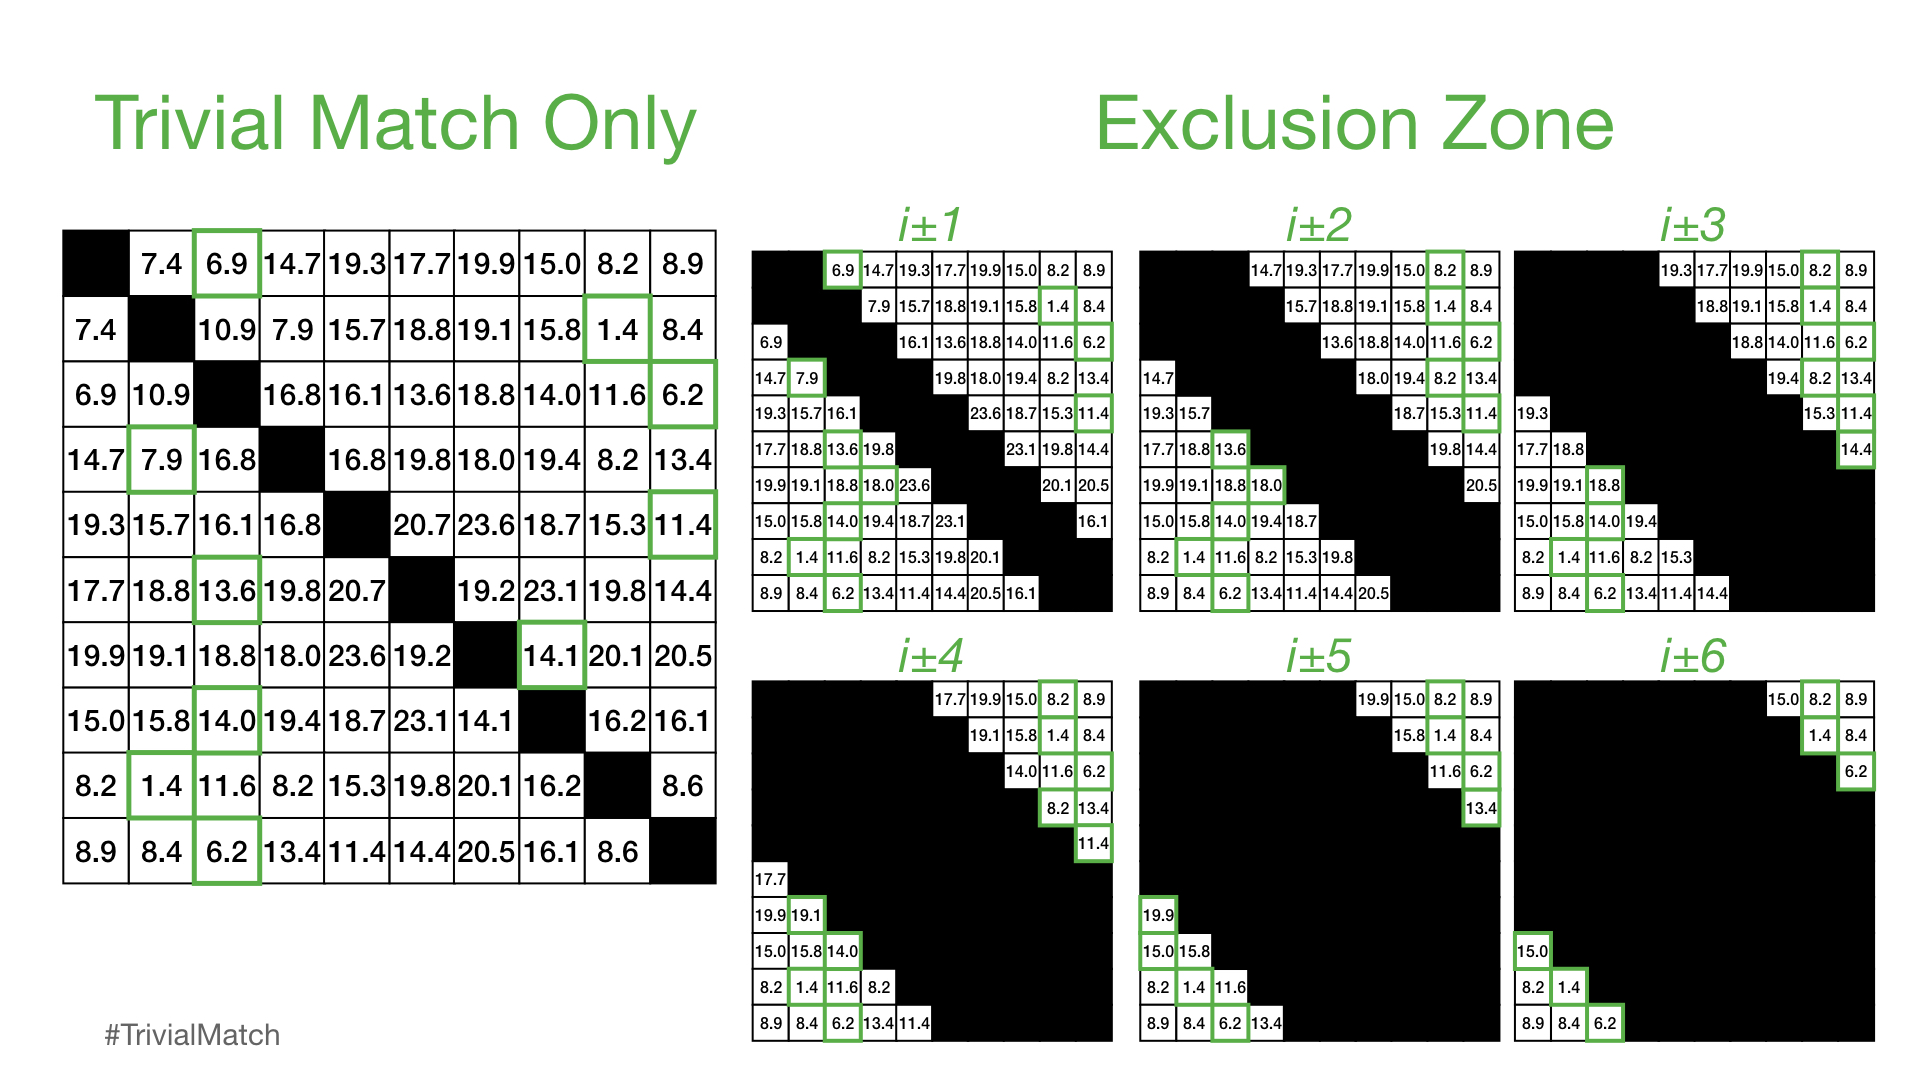
\includegraphics[scale=0.25]{exclusion_zone.jpg}
\caption{Exclusion Zone Sizes}
\label{fig:ExclusionZone}
\end{center}
\end{figure*}

We want to find the nearest neighbor for every subsequence of $T$.  The nearest neighbor information is store in two meta time series, the \emph{Matrix Profile} and the \emph{Matrix Profile Index}:

\textbf{Definition 4:} A \emph{Matrix Profile} $P$ of time series $T$ is a vector of the Euclidean distances between every subsequence of $T$ and its nearest neighbor in $T$.  Formally, $P$ = [min($D_1$), min($D_2$), \ldots{}, min($D_{n-m+1}$)], where $D_i(1 \leq i \leq n-m+1)$ is the distance profile $D_i$ corresponding to the query subsequence $T_{i,m}$ and time series $T$.

The $i^{th}$ element of the Matrix Profile gives the Euclidean distance from the query subsequence $T_{i,m}$ to its nearest neighbor in time series $T$.  However, it does not give the \emph{location} of that nearest neighbor; this information is stored in the \emph{Matrix Profile Index}:

\textbf{Definition 5:} A \emph{Matrix Profile Index} $I$ of time series $T$ is an integer vector: $I = [I_1, I_2, \ldots{}, I_{n-m+1}]$, where $I_i = j$ if $d_{i,j}$ = min($D_i$).

Figure~\ref{fig:DistanceProfilesIntoMatrixProfile} illustrates the relationship between distance profiles and the Matrix Profile.  Each row in the distance matrix is a distance profile.  The minimum of each column is selected and collected in the Matrix Profile.  (The diagonal and the exclusion zone immediately around it are ignored.)  The Matrix Profile Index stores the location where the minimum of that column was found\cite{MatrixProfile14}.

\begin{figure}
\begin{center}
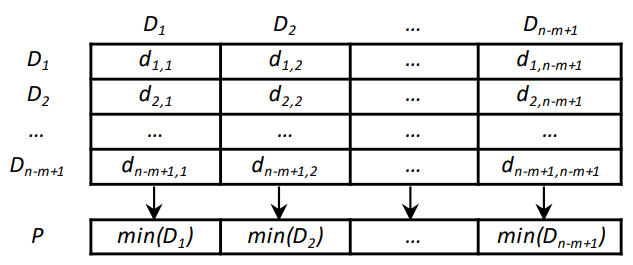
\includegraphics[scale=0.40]{distance_profiles_into_matrix_profile.png}
\caption{Distance Profile Minima Collected into Matrix Profile}
\label{fig:DistanceProfilesIntoMatrixProfile}
\end{center}
\end{figure}

Each distance matrix element $d_{i,j}$ is the distance between $T_{i,m}$ and $T_{j,m} (1 \leq i, j \leq n-m+1)$ of time series $T$.  Figure~\ref{fig:DefinitionsIllustrated} shows an example time series and how the above definitions might be visualized\cite{MatrixProfile11}.  These definitions present the Matrix Profile as a \emph{self-join}.  That is, for every subsequence in a time series $T$, we find its non-trivial-match nearest neighbor within the \emph{same} time series.  To be more broadly useful, the Matrix Profile can be extended to be an AB-join: for every subsequence in a time series $A$, find the nearest neighbors in time series $B$ \cite{MatrixProfile2}\cite{MatrixProfile14}.  For the purposes of this project, we will only deal with the self-join scenario.

\begin{figure}
\begin{center}
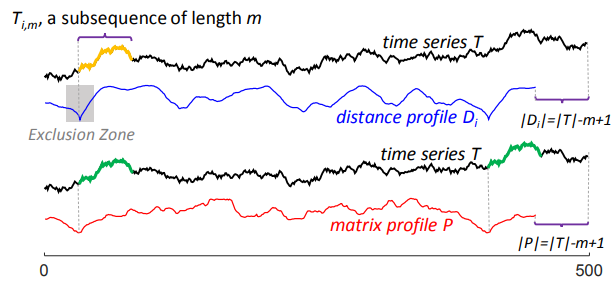
\includegraphics[scale=0.40]{definitions_illustrated.png}
\caption{Definitions Illustrated}
\label{fig:DefinitionsIllustrated}
\end{center}
\end{figure}

\section{Approach}
The Matrix Profile has revolutionized time series data mining tasks and has been heavily optimized, improved, and enhanced since it was announced in 2016.  At the time of this project (2022), there are twenty-three Matrix Profile papers\cite{Keogh} and many Matrix Profile algorithms: STAMP, STAMP\emph{I}, STOMP, SCRIMP, SCRIMP++, SWAMP, and GPU-STOMP.  This project uses the original STAMP algorithm described in the first Matrix Profile paper\cite{MatrixProfile1} with an aim for simplicity in implementation.

The MPI implementation strategy for Matrix Profile is fairly simple for time series data that will fit in the working memory of the MPI processor computers.  
\begin{enumerate}
    \item Leader (rank 0) MPI process parses and validates command line arguments to get an input time series filename, an output matrix profile filename, a subsequence window size, and an input time series column (time series data is frequently stored in comma-separated value formats).
    \item Leader MPI process reads in time series data from the specified input file.
    \item Leader MPI process \texttt{MPI\_Bcast}s time series data to all other processes.
    \item Each MPI process works on distance profile calculations for a segment of time series indices (values of $i$) based on their MPI process rank.  For example, if there are 4 MPI processes, then rank 0 will work on the first fourth of the indices, rank 1 will work on the second fourth of the indices and so forth. 
    \item Each MPI process maintains its own local Matrix Profile and local Matrix Profile Index consisting of the minima and indices of the distance profiles it calculates.  Each time a distance profile is calculated, it is merged into the local Matrix Profile by performing an element-wise minimum with the exception of the trivial match and the surrounding exclusion zone.
    \item After each non-Leader MPI process finishes its segment of time series indices, it \texttt{MPI\_Send}s its local Matrix Profile and local Matrix Profile Index to the Leader (rank 0) process.
    \item After the Leader process finishes its segment of the time series indices, it \texttt{MPI\_Recv}s the local Matrix Profiles and local Matrix Profile Index from the other processes.  For each received local Matrix Profile and local Matrix Profile Index, the Leader process merges the received Matrix Profile and Index into its own using the same element-wise minimum algorithm used to merge a distance profile into the local Matrix Profile.
    \item Once all the other processes' local Matrix Profiles and Indices have been merged, the Leader process writes the final Matrix Profile to the output file.
\end{enumerate}

\section{Simulation}
There are no simulations for this project.

\section{Tests}
In order to validate the finished MPI implementation of Matrix Profile in C++ a test suite was created.  The test suite contains nine input time series and their corresponding matrix profiles.  The STUMPY\cite{Stumpy} Python library implementation of the Matrix Profile was used to process the input time series and the output Matrix Profile data structures were captured.  The MPI Matrix Profile implementation was validated as correct because the output Matrix Profile data structures match those created by the STUMPY Matrix Profile implementation. 

Additionally, unit tests were created to validate that each component of the MPI Matrix Profile implementation works as expected.  GitHub Actions were also used to perform multi-platform (Linux, MacOS, and Windows) builds and unit tests before pull requests were allowed to merge into the \texttt{main} branch.  See https://github.com/rmcnew/parallel\_group\_project/actions for more information.

\section{Test Datasets}
Real world time series data was used in the test suite.  Figures~\ref{fig:AAPL_time_series} through ~\ref{fig:GDP_time_series} show the input test time series datasets and a brief description of each.  Note that many of the time series used are relatively small compared to some real world time series data which range up to multiple gigabytes in size for rapidly generated or multivariate data.  The number of datapoints for each time series is given in each figure caption to show its size.

%\begin{figure*}
%\begin{center}
%\caption{Test Dataset Input Time Series Data}
%\begin{tabular}{|c|c|c|}
%\hline
%\textbf{Filename} & \textbf{Datapoints} & \textbf{Description} \\ \hline \hline
%AAPL.csv & 254 & Apple stock daily adjusted close price from 2021-02-11 to 2022-02-11 \\ \hline
%AirPassengers.csv & 144 & Monthly airline passengers from 1949 to 1960 \\ \hline
%AMZN.csv & 6228 & Amazon stock daily adjusted close price from 1997-05-15 to 2022-02-10 \\ \hline
%california\_covid19\_cases.csv & 740 & Daily California COVID-19 cases from 2020-02-01 to 2022-02-09 \\ \hline
%daily\_min\_temperature.csv & 3649 & Daily minimum temperatures from 1981-01-01 to 1990-12-31  \\ \hline
%jena\_climate\_2009\_2016.csv & 420551 & Jena, Germany temperatures from 2009-01-01 to 2017-01-01  \\ \hline
%MSFT.csv & 254 & Microsoft stock daily adjusted close price from 2021-02-11 to 2022-02-11 \\ \hline
%TSLA.csv & 253 & Tesla stock daily adjusted close price from 2021-02-11 to 2022-02-10 \\ \hline
%us\_gdp.csv & 300 & US quarterly GDP from 1947-01-01 to 2021-10-01 \\ \hline
%\hline
%\end{tabular}
%\label{fig:Input_Time_Series}
%\end{center}
%\end{figure*}

\begin{figure*}
\begin{center}
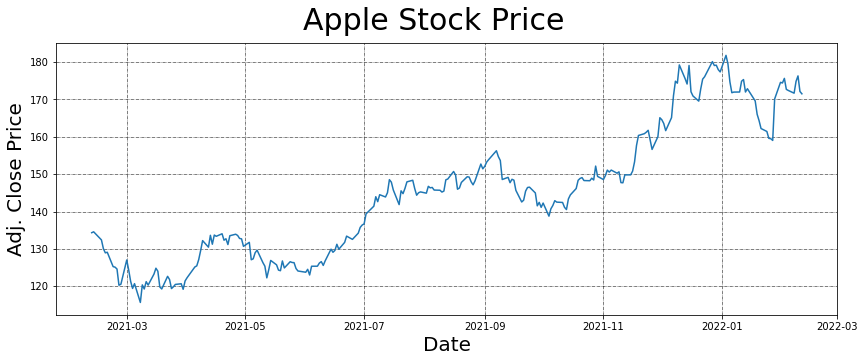
\includegraphics[scale=0.42]{AAPL_time_series.png}
\caption{Apple stock daily adjusted close price from 2021-02-11 to 2022-02-11, 254 datapoints}
\label{fig:AAPL_time_series}
\end{center}
\end{figure*}

\begin{figure*}
\begin{center}
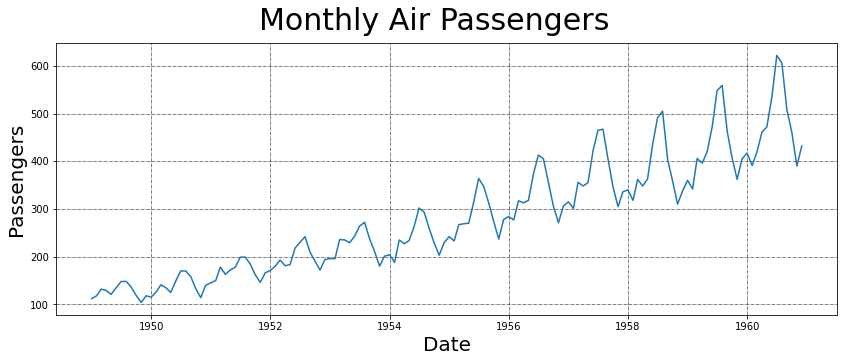
\includegraphics[scale=0.42]{AirPassengers_time_series.png}
\caption{Monthly airline passengers from 1949 to 1960, 144 datapoints}
\label{fig:AirPassengers_time_series}
\end{center}
\end{figure*}

\begin{figure*}
\begin{center}
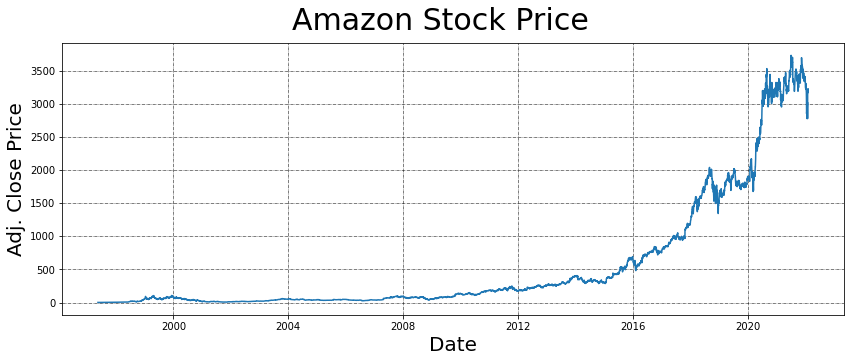
\includegraphics[scale=0.42]{AMZN_time_series.png}
\caption{Amazon stock daily adjusted close price from 1997-05-15 to 2022-02-10, 6228 datapoints}
\label{fig:}
\end{center}
\end{figure*}

\begin{figure*}
\begin{center}
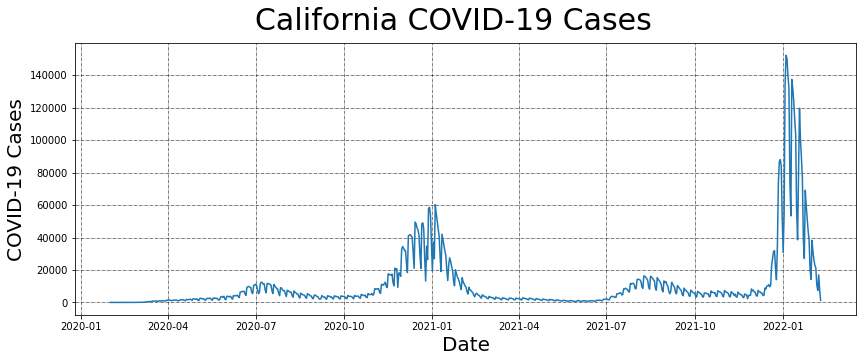
\includegraphics[scale=0.42]{CA_COVID19_time_series.png}
\caption{Daily California COVID-19 cases from 2020-02-01 to 2022-02-09, 740 datapoints}
\label{fig:CA_COVID19_time_series}
\end{center}
\end{figure*}

\begin{figure*}
\begin{center}
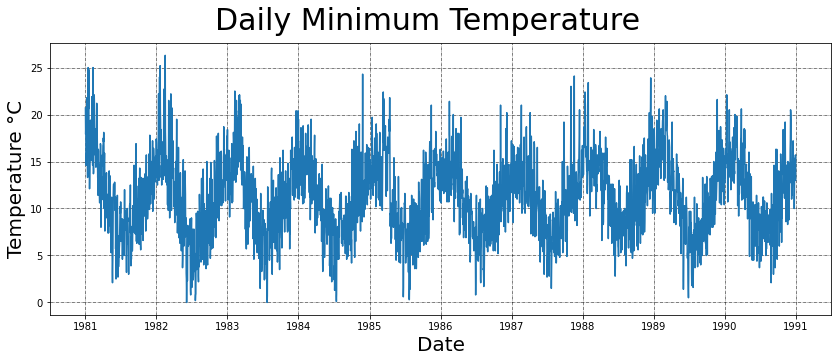
\includegraphics[scale=0.42]{DailyMinTemp_time_series.png}
\caption{Daily minimum temperatures from 1981-01-01 to 1990-12-31, 3649 datapoints}
\label{fig:DailyMinTemp_time_series}
\end{center}
\end{figure*}

\begin{figure*}
\begin{center}
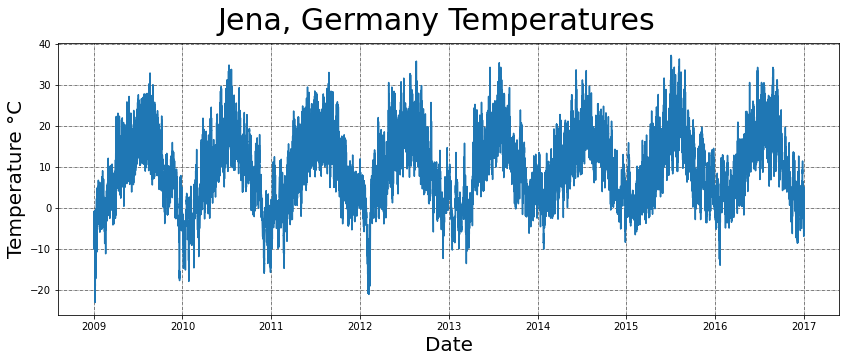
\includegraphics[scale=0.42]{Jena_time_series.png}
\caption{Jena, Germany temperatures from 2009-01-01 to 2017-01-01, 420551 datapoints}
\label{fig:Jena_time_series}
\end{center}
\end{figure*}

\begin{figure*}
\begin{center}
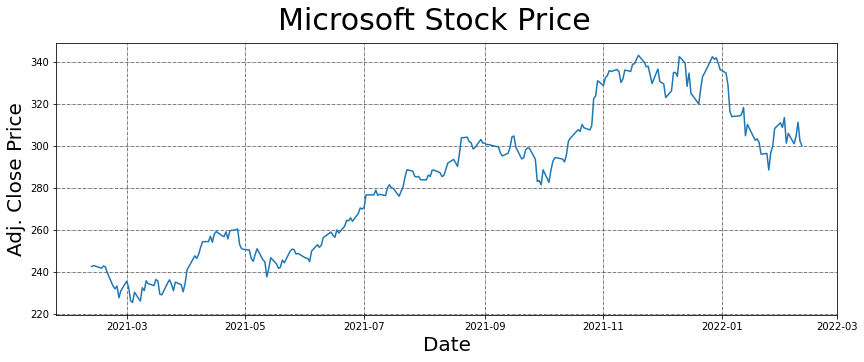
\includegraphics[scale=0.42]{MSFT_time_series.png}
\caption{Microsoft stock daily adjusted close price from 2021-02-11 to 2022-02-11, 254 datapoints}
\label{fig:MSFT_time_series}
\end{center}
\end{figure*}

\begin{figure*}
\begin{center}
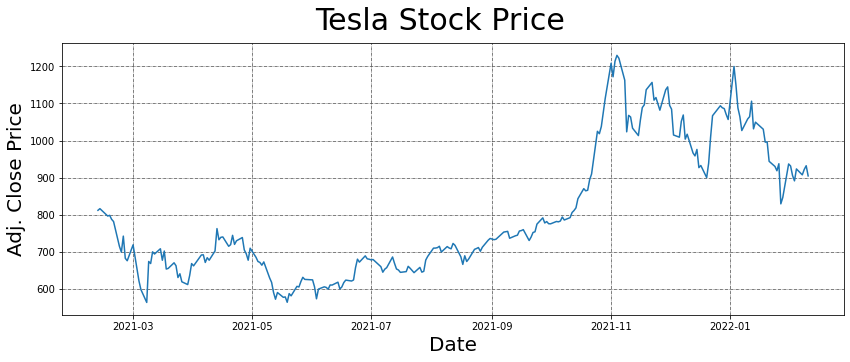
\includegraphics[scale=0.42]{TSLA_time_series.png}
\caption{Tesla stock daily adjusted close price from 2021-02-11 to 2022-02-10, 253 datapoints}
\label{fig:TSLA_time_series}
\end{center}
\end{figure*}

\begin{figure*}
\begin{center}
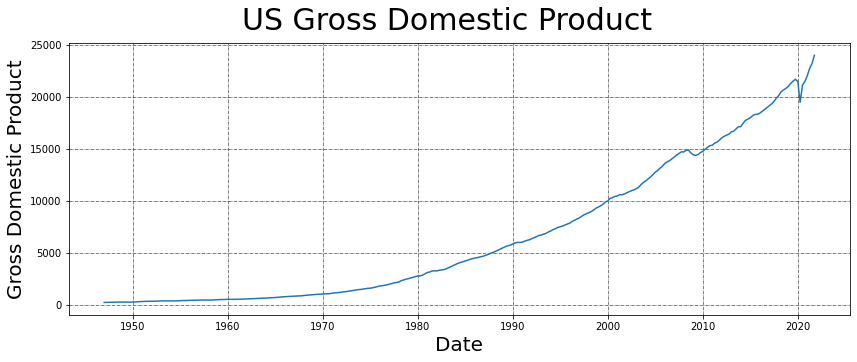
\includegraphics[scale=0.42]{GDP_time_series.png}
\caption{US quarterly GDP from 1947-01-01 to 2021-10-01, 300 datapoints}
\label{fig:GDP_time_series}
\end{center}
\end{figure*}


\section{Results}

The MPI Matrix Profile implementation calculated the same results as the STUMPY Matrix Profile implementation with 99.95\% similarity.  Figure~\ref{fig:Matrix_Profile_Percent_Similarity} lists the percent similarity for each input time series matrix profile. 

\begin{figure*}
\begin{center}
\caption{Test Dataset Output Matrix Profile Percent Similarity}
\begin{tabular}{|c|c|}
\hline
\textbf{Filename} & \textbf{Percent Similarity} \\ \hline \hline
AAPL\_matrix\_profile.csv & 99.99 \\ \hline
AMZN\_matrix\_profile.csv & 99.99 \\ \hline
AirPassengers\_matrix\_profile.csv & 100.00 \\ \hline
california\_covid19\_cases\_matrix\_profile.csv & 99.99 \\ \hline
daily\_min\_temperature\_matrix\_profile.csv & 99.99 \\ \hline
jena\_climate\_2009\_2016\_matrix\_profile.csv & N/A \\ \hline
MSFT\_matrix\_profile.csv & 99.99 \\ \hline
TSLA\_matrix\_profile.csv & 99.60 \\ \hline
us\_gdp\_matrix\_profile.csv & 99.99 \\ \hline \hline
Overall Percent Difference & 99.95 \\ \hline
\hline
\end{tabular}
\label{fig:Matrix_Profile_Percent_Similarity}
\end{center}
\end{figure*}

The percent similarity calculations were performed as the inverse of the percent difference: $percent\_similarity = \left(1 - \frac{|actual - expected|}{expected}\right) * 100$ where the $expected$ values were those provided by the STUMPY matrix profile output and the $actual$ values were those provided by our MPI matrix profile output. Note that no percent similarity is given for the Jena climate time series because the MPI implementation ran for several days, but never finished.  This is likely due to the size of the time series and the less efficient STAMP algorithm.

Figure~\ref{fig:Matrix_Profile_Diff} shows an example side-by-side difference comparison between two output matrix profiles.  The left side is the STUMPY Python library output.  The right side is the MPI C++ Matrix Profile output.  This figure illustrates how similar most of the matrix profile output was between the STUMPY implementation and our MPI implementation out to many decimal places.

\begin{figure*}
\begin{center}
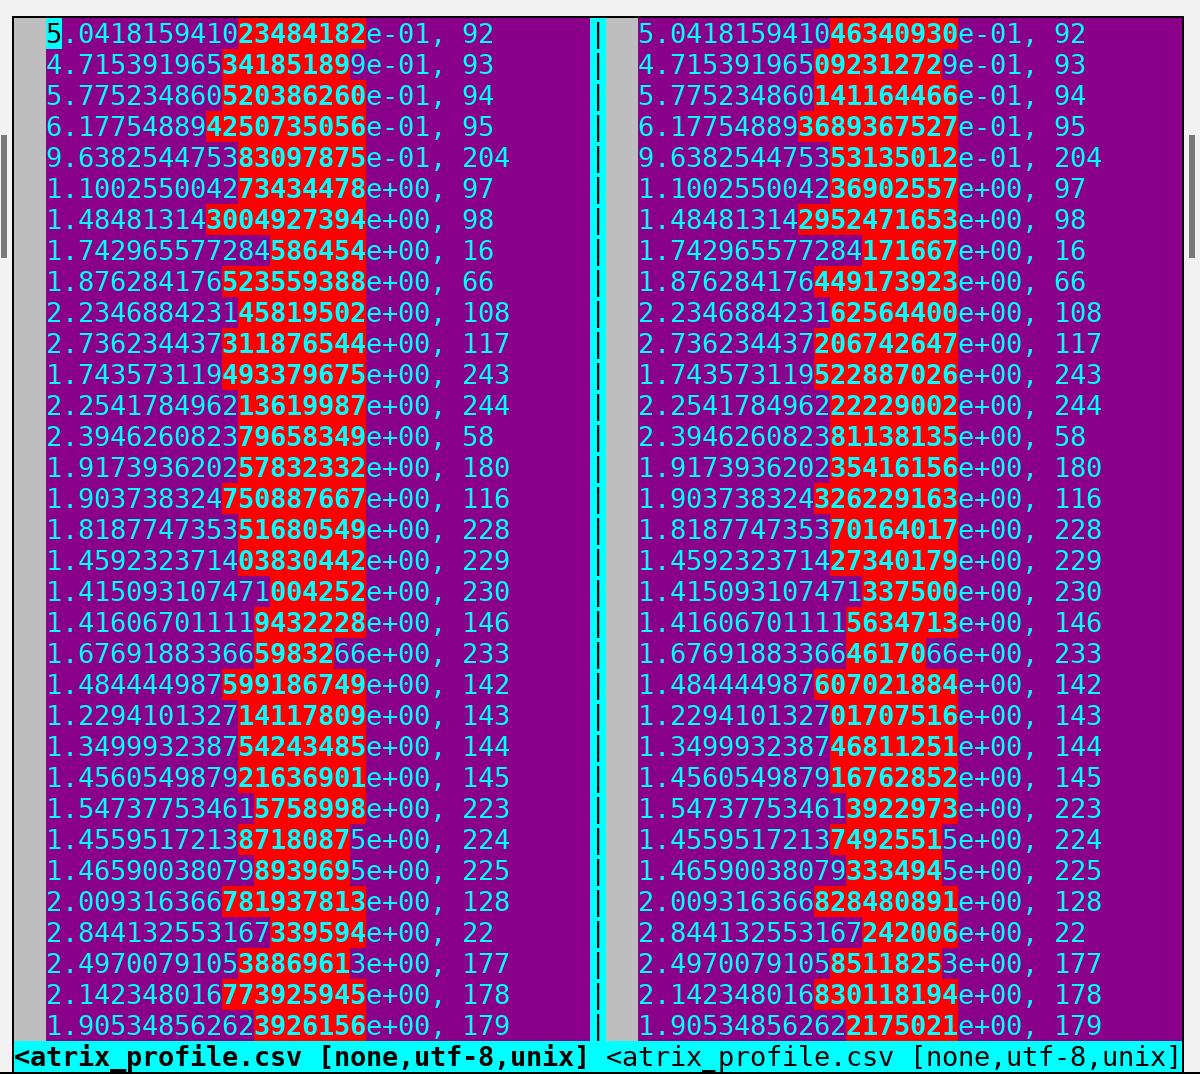
\includegraphics[scale=0.42]{matrix_profile_diff.png}
\caption{Side-by-side difference comparison between matrix profile output.   Left: STUMPY Python output, Right: MPI C++ output}
\label{fig:Matrix_Profile_Diff}
\end{center}
\end{figure*}

\section{Performance Comparison}

A simple performance comparison test was run to compare the execution time, CPU utilization, and memory usage between the reference STUMPY Python matrix profile implementation and our MPI C++ implementation.  These performance tests were run on a Intel Core i5-5250 processor with four cores and 16 GB RAM running Debian Linux with version 5.15.23 of the Linux kernel.  

Note that this comparison is not fair for two reasons:  1) the STUMPY library uses a just-in-time optimized version of the STOMP matrix profile algorithm\cite{Stumpy} whereas our MPI C++ implementation uses the original, less optimized STAMP matrix profile algorithm\cite{MatrixProfile1}, and 2) comparing a serial Python program against a parallelized C++ program is unfair due to the massive difference in language runtimes.  The differences are apparent in the performance comparison results. 

%\begin{figure*}
%\begin{center}
%\caption{Execution Time in Seconds}
%\begin{tabular}{|c|c|c|}
%\hline
%\textbf{Input Filename} & \textbf{STUMPY Python} & \textbf{MPI C++} \\ \hline \hline
%AAPL.csv & 15.27 & 0.09 \\ \hline
%AMZN.csv & 15.67 & 21.70 \\ \hline
%AirPassengers.csv & 15.14 & 0.04 \\ \hline
%california\_covid19\_cases.csv & 15.13 & 0.24 \\ \hline
%daily\_min\_temperature.csv & 15.38 & 5.19 \\ \hline
%jena\_climate\_2009\_2016.csv & 642.67 & N/A \\ \hline
%MSFT.csv & 15.14 & 0.08 \\ \hline
%TSLA.csv & 15.22 & 0.07 \\ \hline
%us\_gdp.csv & 15.27 & 0.08 \\ \hline \hline
%\end{tabular}
%\label{fig:Execution_Time}
%\end{center}
%\end{figure*}

The MPI matrix profile implementation is easily faster than the STUMPY matrix profile implementation for time series with a smaller number of datapoints, but is much slower for larger time series.  This is due to the more efficient STOMP algorithm that STUMPY uses compared to the MPI implementation's STAMP algorithm.  Note that the Jena climate time series is incomplete because our MPI implementation ran for several days but did not finish the computation.  Figure~\ref{fig:Time_Graph} displays how many seconds it took the Python and C++ code to complete the matrix profile calculations.

\begin{figure*}
\begin{center}
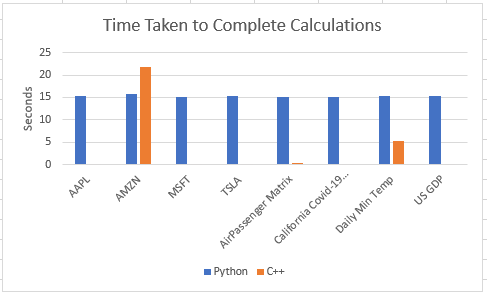
\includegraphics[scale=1.05]{Time.png}
\caption{Compares how many seconds it took the Python code and C++ code to complete the matrix profile calculations}
\label{fig:Time_Graph}
\end{center}
\end{figure*}

%\begin{figure*}
%\begin{center}
%\caption{Percent CPU Utilization}
%\begin{tabular}{|c|c|c|}
%\hline
%\textbf{Input Filename} & \textbf{STUMPY Python} & \textbf{MPI C++} \\ \hline \hline
%AAPL.csv & 106\% & 338\% \\ \hline
%AMZN.csv & 108\% & 398\% \\ \hline
%AirPassengers.csv & 106\% & 308\% \\ \hline
%california\_covid19\_cases.csv & 106\% & 374\% \\ \hline
%daily\_min\_temperature.csv & 107\% & 397\% \\ \hline
%jena\_climate\_2009\_2016.csv & 385\% & N/A \\ \hline
%MSFT.csv & 106\% & 335\% \\ \hline
%TSLA.csv & 106\% & 330\% \\ \hline
%us\_gdp.csv & 106\% & 331\% \\ \hline \hline
%\end{tabular}
%\label{fig:CPU_Utilization}
%\end{center}
%\end{figure*}

For CPU Utilization, the STUMPY implementation only uses one CPU core for most of the time series compared to the MPI implementation using all available CPU cores.  However, STUMPY does use multiple cores for the large Jena climate time series.  This is due to STUMPY using the Numba just-in-time (JIT) compiler Python library that translates a subset of Python and NumPy code into native machine code.  Numba supports automatic conversion of array expressions into parallel code\cite{Numba}, thus the higher CPU utilization for the larger Jena climate time series.  Figure~\ref{fig:CPU_Graph} gives the CPU usage percentage. 100\% means 1 core, 300\% means 3 cores were used.

\begin{figure*}
\begin{center}
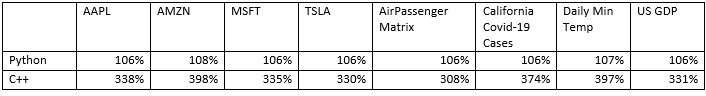
\includegraphics[scale=1.05]{CPU.png}
\caption{CPU usage percentage. 100\% means 1 core, 300\% means 3 cores were used.}
\label{fig:CPU_Graph}
\end{center}
\end{figure*}

%\begin{figure*}
%\begin{center}
%\caption{Memory Usage in Kilobytes}
%\begin{tabular}{|c|c|c|}
%\hline
%\textbf{Input Filename} & \textbf{STUMPY Python} & \textbf{MPI C++} \\ \hline \hline
%AAPL.csv & 219572 & 13680 \\ \hline
%AMZN.csv & 222204 & 16276 \\ \hline
%AirPassengers.csv & 219816 & 13284 \\ \hline
%california\_covid19\_cases.csv & 220040 & 13280 \\ \hline
%daily\_min\_temperature.csv & 221240 & 14548 \\ \hline
%jena\_climate\_2009\_2016.csv & 431388 & N/A \\ \hline
%MSFT.csv & 220040 & 13580 \\ \hline
%TSLA.csv & 220116 & 13316 \\ \hline
%us\_gdp.csv & 220452 & 13360 \\ \hline \hline
%\end{tabular}
%\label{fig:Memory_Usage}
%\end{center}
%\end{figure*}
The STUMPY matrix profile implementation uses about fifteen times as much memory as our MPI implementation on average.  This is expected given that STUMPY runs in a heavier garbage-collected Python runtime and with a Numba JIT compiler compared to the far more minimal C++ environment and MPI C library. Figure~\ref{fig:Memory_Graph} shows the amount of memory in kilobytes that the Python and C++ programs used.
\begin{figure*}
\begin{center}
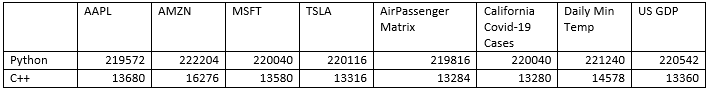
\includegraphics[scale=1.05]{Memory.png}
\caption{The amount of memory in kilobytes the Python and C++ programs used.}
\label{fig:Memory_Graph}
\end{center}
\end{figure*}
\section{Conclusion}
In this project we created a minimal MPI-based implementation of the Matrix Profile in C++.  It works very well for time series with a small number of datapoints, but does not scale up well to larger time series.  This is primarily due to our use of the original STAMP algorithm which is much slower than the STOMP and SCRIMP++ algorithms. Figure~\ref{fig:matrix_profile_algorithms_compared} gives a graphical comparison of the STAMP algorithm's performance against the STOMP and SCRIMP++ algorithms.  While the STOMP and SCRIMP++ algorithms are much more performant compared to STAMP, they are also much more complex to implement which is why we chose to implement STAMP for this project. 

\begin{figure*}
\begin{center}
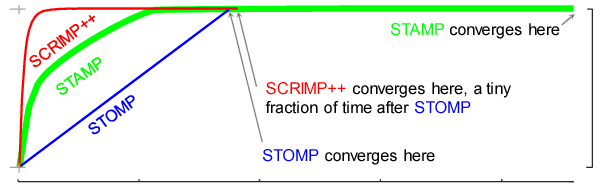
\includegraphics[scale=0.85]{matrix_profile_algorithms_compared.png}
\caption{Matrix Profile algorithms convergence times compared}
\label{fig:matrix_profile_algorithms_compared}
\end{center}
\end{figure*}

\section{Future Work}
The Matrix Profile is an exciting area of research for time series data mining.  Most of the work is focused on mining massive time series datasets as fast as possible in cloud computing environments.  Considering how versatile the Matrix Profile is and how ubiqitous multicore processors are, there is likely a need for a fast, resource-frugal implementation of the Matrix Profile for use in portable and embedded devices such as on-board vehicle computers, field diagnostic medical equipment, smartphones, and industrial control computers.  

An MPI-based implementation similar to (or perhaps derived from) our implementation could be created to use a more optimal Matrix Profile algorithm such as SCRIMP++ and outfitted with a focused domain-specific motif search set in order to quickly search an incoming data stream (time series) for matching subsequences of interest.  For example, an on-board vehicle computer could use sensor data to rapidly recognize a hazardous road condition and alert the driver.  Field diagnostic medical devices could aid doctors or first responders in quickly finding life-threatening diseases so that the proper care can be given with minimal delay.  Smartphones could gain even more capabilities with on-device sensors that identify emergencies and request help (e.g. active shooter situations, explosions, car accidents, et cetera).  Industrial control computers could better respond to their environment by sensing failure conditions and shutting down production to prevent injuries and loss of expensive equipment.  

There are many possible applications for a fast, resource-frugal, parallel implementation of the Matrix Profile.  This project showed that a minimal MPI Matrix Profile implementation is possible and can be made practical with more effort.

\bibliographystyle{IEEEtran}

% number is the number of reference labels
\begin{thebibliography}{8}  

\bibitem{MatrixProfile1} C. M. Yeh et al., "Matrix Profile I: All Pairs Similarity Joins for Time Series: A Unifying View That Includes Motifs, Discords and Shapelets," 2016 IEEE 16th International Conference on Data Mining (ICDM), 2016, pp. 1317-1322, doi: 10.1109/ICDM.2016.0179.

\bibitem{MatrixProfile2} Y. Zhu et al., "Matrix Profile II: Exploiting a Novel Algorithm and GPUs to Break the One Hundred Million Barrier for Time Series Motifs and Joins," 2016 IEEE 16th International Conference on Data Mining (ICDM), 2016, pp. 739-748, doi: 10.1109/ICDM.2016.0085.

\bibitem{MatrixProfile11} Y. Zhu et al., "Matrix Profile XI: SCRIMP++: Time Series Motif Discovery at Interactive Speeds," 2018 IEEE International Conference on Data Mining (ICDM), 2018, pp. 837-846, doi: 10.1109/ICDM.2018.00099.

\bibitem{MatrixProfile14} Z. Zimmerman et al., "Matrix Profile XIV: Scaling Time Series Motif Discovery with GPUs to Break a Quintillion Pairwise Comparisons a Day and Beyond," 2019 ACM Symposium, pp. 74-86. doi: 10.1145/3357223.3362721. 

\bibitem{DynamicTimeWarping} T. Rakthanmanon et al., "Searching and Mining Trillions of Time Series Subsequences under Dynamic Time Warping," In Proceedings of the 18th ACM SIGKDD international conference on Knowledge discovery and data mining (KDD '12). 2012. Association for Computing Machinery, New York, NY, USA, 262–270. DOI:https://doi.org/10.1145/2339530.2339576.

\bibitem{Stumpy} S.M. Law, (2019). "STUMPY: A Powerful and Scalable Python Library for Time Series Data Mining," Journal of Open Source Software, 4(39), 1504. [Online]. Available: https://github.com/TDAmeritrade/stumpy.

\bibitem{Keogh} E. Keogh, \emph{The UCR Matrix Profile Page}, 2021. [Online]. Available: https://www.cs.ucr.edu/~eamonn/MatrixProfile.html.

\bibitem{Numba} \emph{Numba}, 2022. [Online]. Available: https://numba.pydata.org/.

\end{thebibliography}

\end{document}
